

\chapter{Tobii Sono Flex}

I dette kapittelet vil den eksisterende løsningen sono flex bli diskutert. Det vil bli gitt en grundig analyse av problemstillingen og fremgangsmåte presentert.


\section{Tobii Sono Flex}
\label{chap:Tobii-Sono-Flex}


Programvaren som det tas utgangspunkt i heter Tobii Sono Flex,  og er et systematisert symbolforråd og et verktøy for alternativ og supplerende symbolspråk. Sono Flex har som mål å tilby et språk til personer som ikke enda kan lese og skrive. 

Applikasjonen fungerer som et tastatur, men istedenfor bokstaver er knappene ord med en visuell representasjon av ordet. Brukeren trykker på knappene som utgjør setningen han vil uttrykke, så vil programvaren gjøre om setningen til tydelig tale.  Systemet er spesielt utviklet for barn og unge med med sammensatte kommunikasjonsvansker, som trenger et ordforråd for å videreutvikle språk- og kommunikasjonsferdigheter. Sono flex kan ses på som en nybegynnerpakke med en lav læringskurve som skal gjøre brukeren klar for mer avanserte systemer. 


\subsection{Brukergrensesnitt}

Brukergrensesnittet til Sono Slex består av to hovedkomponenter: en menylinje og en symboltabell. 


\subsubsection{Menylinje}

Figur \ref{fig:menylinje} viser menylinjen.  Denne består av 5 elementer.  Kun de midterste er av interesse, disse  er statiske og følger applikasjonen hele tiden. Det hvite feltet i midten viser symbolene som brukerene har trykket på, og vil herved bli referert til som setningslisten. Symbolene som vises vil komme ut i form av tydelig tale ved å trykke på selve feltet. Knappen på venstre side av setningslisten (clear all), vil ved interaksjon tømme setningslisten. Mens knappen på høyre side vil kun fjerne det siste symbolet brukeren trykket på.


\begin{figure}[ht!]
\centering
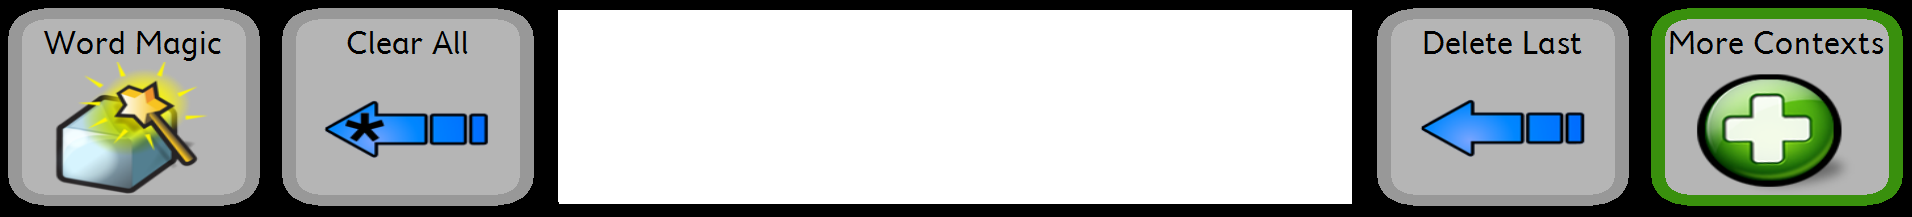
\includegraphics[width=100mm]{menylinje}
\caption{Skjermdump av menylinjen til programvaren Sono Flex}
\label{fig:menylinje}
\end{figure}




\subsubsection{symboltabell}
\label{subsubsec:symboltabell}

Figur \ref{fig:symbolgrid} viser applikasjonens symboltabell. Dette komponentet består av en tabell på 7 kolonner og 4 rader,  noe som gir 28 celler. I hver celle er det et Knapp bestående av et symbol og en tekstlig beskrivelse av symbolet. Ved å trykke på knappen vil en av tre ting skje avhengig av hvilken type knappen er av. Hvis knappen representerer et ord( "jeg",  "løpe",  "kake" o.s.v. ) så vil symbolet og medfølgende tekst vises i setningslisten i menylinje.  Hvis knappen har underliggende knapper som eksempelvis en ordklasse(verb,  substantiv)  eller kategori ("mat",  "frukt") så vil applikasjonen bytte ut de eksisterende symbolene i tabellen med ordene i ordklassen. Den siste typen symbol, er et navigasjonssymbol. Denne forekommer kun hvis det er for mange symboler i forhold til hvor mange det er plass til. Eksempelvis er det plass 28 symboler i tabellen, hvis da en kategori inneholder mer enn dette vil disse måtte fordeles over flere sider. Navigasjonssymbolet vil da være representert for å kunne bla mellom de ulike sidene.


\begin{figure}[ht!]
\centering
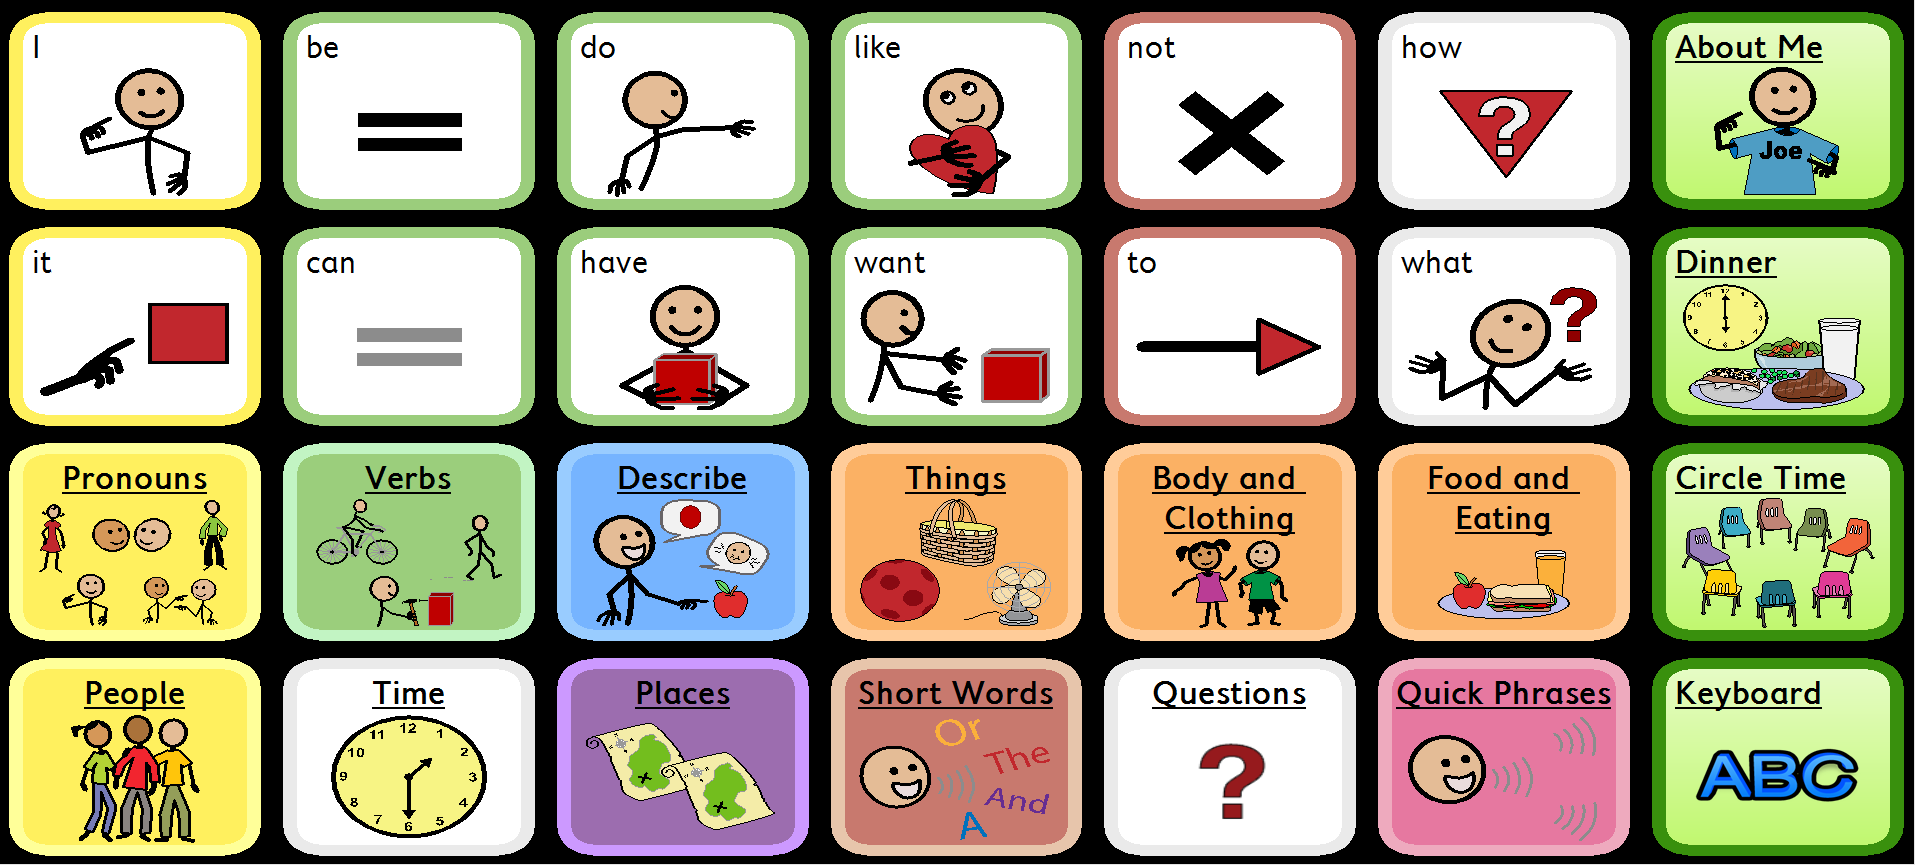
\includegraphics[width=100mm]{symbolgrid}
\caption{Skjermdump av symboltabellen til programvaren Sono Flex}
\label{fig:symbolgrid}
\end{figure}


\subsection{Brukerinteraksjon}

Sono Flex tilbyr to måter for brukerinteraksjon,  mus og øyestyring. Mus fungerer som vanlig ved at brukeren svever med musepekeren over ønsket knapp og venstreklikker for å aktivere. Ved øyestyring må brukeren fokusere blikket på ønsket knapp en gitt tid for at applikasjonen skal tolke det som et klikk. 

Det som skjer er at med engang brukeren fokuserer blikket på en knapp så starter en nedtelling. Figur \ref{fig:knapp-interaksjon} viser hvordan brukeren presenteres for hvor mye av nedtellingen som gjenstår.  Hvis brukeren ikke flytter blikket før nedtellingen har nådd null tolkes dette som et klikk.
For å gi brukeren beskjed om et godkjent klikk så dannes det en rød firkant rundt knappen. 

\begin{figure}[ht!]
\centering
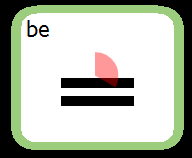
\includegraphics[width=50mm]{Knapp-interaksjon}
\caption{Skjermdump som viser hvordan nedtellingen på en knapp ser ut. Når den røde sirkelen er komplett oppfattes det som et klikk}
\label{fig:knapp-interaksjon}
\end{figure}


\section{Organisasjon og Navigasjon}

Som nevnt i seksjon \ref{subsec:navigasjon} så vil et barns vokabular være så stort at en nødvendigvis må fordele ordene over flere sider. Sono Flex har eksempelvis 106 ord under kategorien "Ting". Med tanke på at det maksimalt er plass til 28 ord på hver side så må disse fordeles og det må finnes en måte å navigere sidene. Løsningen har blitt en svært flat struktur med et hierarki på maksimalt 2 nivåer, ergo det finnes ikke underkategorier. Figur \ref{fig:hieraki-ting} viser hvordan dette fungerer i praksis. Når man trykker på kategorien "ting" så fylles tabellen med 27 ord som passer inn i kategorien "ting". Hvis man ikke finner ønsket ord på den første siden, navigerer man videre med knappen "neste side" og ordene i tabellen erstattes av nye ord. 


\begin{figure}[ht!]
\centering
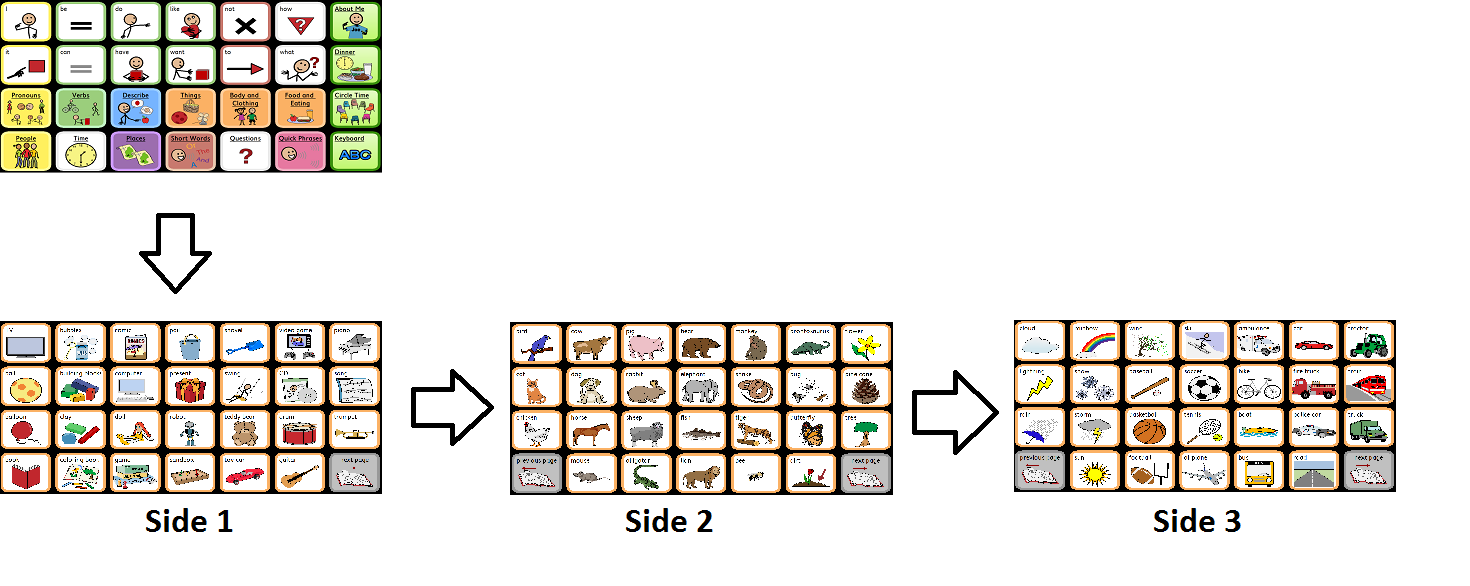
\includegraphics[width=140mm]{Symbgrid}
\caption{Skjermdump hierakiet til Sono Flex}
\label{fig:hieraki-ting}
\end{figure}
